\input{Packages}
\input{Definitions}
\DeclareRobustCommand{\stirling}{\genfrac\{\}{0pt}{}}
%this removes numbering from the section, from some reason the \section*{} command doesnt work once you redefine it
\setcounter{secnumdepth}{0} 


\begin{document}
\pagestyle{empty}
\sloppy
\maketitle

\section{Selected Topic: Counting}

\begin{problem}[C][4][AMATYC Fall 2013/15]
    % Counting ^ Student Math League
    All fractions \(0 < \frac{a}{b} < 1\) (where \(a, b\) are positive integers) are placed into the sequence 
    \(
    \frac{1}{2}, \frac{1}{3}, \frac{2}{3}, \frac{1}{4}, \frac{2}{4}, \frac{3}{4}, \dots
    \)
    first by increasing order of denominator, then by increasing order of numerator. Find \( a + b \) for the 2013th element of the sequence.
\end{problem}
\multOpt[5]{$124$}[$125$][$126$][$127$][$128$]

\begin{solution}[A]
    To find the 2013th element, we split our sequence \( \displaystyle \frac{1}{2}, \frac{1}{3}, \frac{2}{3}, \frac{1}{4}, \frac{2}{4}, \frac{3}{4}, \dots \) up by denominator \(b\).
    
    For \(b=2\) we have 1 term, for \(b=3\) we have 2 terms, and for \(b=4\) we have 3 terms. In general, for \(b=k\) we get \(k-1\) terms. This pattern will continue forever because for each \(b\) we increment the numerator, starting from \(1\), until it reaches \(b-1\). Thus by carrying out this process through the \(b\)th denominator, we'll have
    \[
        \frac{\big[b-1\big]\big[(b-1)+1\big]}{2} = \frac{b(b-1)}{2} \,\text{total terms.}
    \]
    Then, setting \(b(b-1)/2 = 2013\) gives us \(b\approx 63.95\), and so we know the 2013th term must have a denominator of 64. To find the exact term, we find that \( 63(62)/2 = 1953\) is the index of the last term with a denominator of \(63\), and since \(2013-1953=60\), our solution will be the 60th term with a denominator of 64---in other words, \(\dfrac{60}{64}\). Thus, \(a+b=60+64=\boxed{124}\).
\end{solution}

\begin{problem}[C][3][AMATYC Fall 2017/20]
    % Counting ^ Student Math League
    How many positive integers less than or equal to 1000 have an equal number of even and odd factors? For example, 10 would be counted since it has two odd (1 and 5) and two even (2 and 10) factors.
\end{problem}
\multOpt[5]{$100$}[$125$][$200$][$250$][$500$]

\begin{solution}[D]
    We can immediately rule out all 500 odd numbers up to 999, since they do not contain any even factors. For the remaining even factors, keep in mind that this problem is talking about \emph{all} factors, not just primes. So we must think about using the prime factorization of a number to create all possible factors.
        
    If the number is divisible by exactly one power of 2 (as opposed to having a factor of \(2^2\) or higher), then using all other possible factors, we can either pair them with the 2 or not pair them with 2, giving us an equal number of even and odd factors. But if the number is divisible by 4, than each odd factor could be paired with either \(2^2\) (both 2s), 2 (just one), or neither to create way more even factors than odd factors. Since half of even numbers are divisible by 4 (these are numbers of the form \( n=2(2k) \), we rule out half of the remaining 500 even numbers under consideration, for a total of \fbox{250} terms with an equal number of even and odd factors.
\end{solution}

\begin{problem}[C][1][AIME 1991/5]
    % Counting ^ AIME
    Given a rational number, write it as a fraction in lowest terms and calculate the product of the resulting numerator and denominator. For how many rational numbers between $0$ and $1$ will $20!$ be the resulting product? 
\end{problem}

\begin{solution}[\(2^7\)]
    We want to know how many fully reduced fractions \(\dfrac{a}{b}\in(0,1)\) have \(a\) and \(b\) such that \( ab = 20! \)

    It's quite easy to think of examples that do and don't work here. For example \(a=20\) and \(b=19!\) don't work, because \(20\) and \(19!\) are both divisible by \(2\), so the fraction wouldn't be reduced. But \(a=19\) and \(b=20\cdot18!\) do work, since \(19\) is prime. However, keep in mind that \(a=20\cdot18!\) and \(b=19\) don't, since \(a>b\).
    
    To determine this, we'll start by determining the prime factors of \(20!\). This is simply all the prime factors of \(1, 2, 3, \dots, 19,  20\), giving us a list of \( 2, 3, 5, 7, 11, 13, 17, 19.\)
    
    We can then simply place these factors on the top or the bottom of the fraction and consider all possible combinations. Now, we don't necessarily know the whole factorization (the powers of each prime factor) of \(20!\)---but since the numerator and denominator have to be coprime (no common factors), we know that if there's a 2 in the numerator, all 2s must also be in the numerator. Otherwise, the fraction could be reduced.

    So how many fractions can be created? Well, for each prime factor, there are 2 possible placements (numerator or denominator), and there are 8 total prime factors, so there are \(2^8\) possible fractions. The only issue with this is that, for example, both \( \frac{20!}{1} \) and \( \frac{1}{20!} \) will be counted. In other words, for each valid solution in our \(2^8\) fractions, its reciprocal---which is definitely \emph{not} valid---will also be counted. To eliminate these cases, we can cut our count in half, dividing by 2 for a total of \(\boxed{2^7}\) rational numbers.
\end{solution}

\begin{problem}[C][2][AIME 2006/6]
    % Counting ^ AIME
    Let $\mathcal{S}$ be the set of real numbers that can be represented as repeating decimals of the form $0.\overline{abc}$ where $a,b,c$ are distinct digits. Find the sum of the elements of $\mathcal{S}$.    
\end{problem}

\begin{solution}[360]
We use the fact that $0.\overline{abc} = \frac{abc}{999}$ where $a$, $b$, and $c$ are distinct digits from $\{0,1,2,\dots,9\}$.

In these arrangements, each digit from $\{0,1,2,\dots,9\}$ appears exactly $72$ times in each position ($a$, $b$, and $c$), since for a given digit in a position, there are $9 \cdot 8 = 72$ ways to fill the remaining positions.

The sum of all elements in $\mathcal{S}$ is therefore:
\[
\sum_{s \in \mathcal{S}} s = \frac{72(0+1+\cdots+9)(100+10+1)}{999} = \frac{72(45)(111)}{999} = \boxed{360}
\]
\end{solution}

\begin{problem}[C][3][AMC 12]
    % Counting ^ Probability ^ AMC
    Flora the frog starts at $0$ on the number line and makes a sequence of jumps to the right. In any one jump, independent of previous jumps, Flora leaps a positive integer distance $m$ with probability $\frac{1}{2^m}$. What is the probability that Flora will eventually land at $10$? 
\end{problem}

\begin{solution}[1/2]
    Any of the possible routes that lead Flora to land at 10 have probability $2^{-10}$. She lands at $k<10$ with probability $2^{-k}$, then she has to travel a distance $10-k$ to land at 10, giving us a probability of $2^{-k} \cdot 2^{k-10}=2^{-10}$.
    
    Now, we just need to count how many routes she could take to get to 10. For each $k<10$, there are two possibilities---we either land at $k$, or we don't. This gives us $2^9$ possible ways to land at $10$, and so the overall probability is $2^9 \cdot 2^{-10} = \boxed{1/2}$.
\end{solution}

\begin{problem}[C][4][2018 AMC 12B/22]
    % Counting ^ Starts and Bars ^ AMC
    Consider polynomials $P(x)$ of degree at most $3$, each of whose coefficients is an element of $\{0, 1, \ldots, 9\}$. How many such polynomials satisfy $P(-1) = -9$?
\end{problem}
\multOpt[5]{110}[143][165][220][286]

\begin{solution}[D]
    We have 
    \[ 
        P(x) = ax^3 + bx^2 + cx + d \quad \Rightarrow \quad P(-1) = -a + b - c + d.
    \]
    Then, to solve \( -a + b - c + d = -9 \), we'll use the stars and bars method. To make all the terms positive, we'll perform the substitutions \( -a = a' - 9 \) and \( -c = c' - 9 \) with \( a', c' \in [0,9]\) (so that \(-a, -c \in [-9,0]\)), giving us
    \[
        a' - 9 + b + c' - 9 + d = -9 \quad \Rightarrow \quad a' + b + c' + d = 9.
    \]
    So we have 3 bars and 9 stars, giving us \( \dbinom{12}{3} = \boxed{220} \) total solutions.
\end{solution}

\begin{problem}[C][7][A Walk Through Combinatorics]
    % Discrete
    A round robin chess tournament had $2n$ participants from two countries, $n$ from each country. There were no two players with the same number of points at the end. Prove that there was at least one player who scored at least as many points against his compatriots as against the players of the other country. (In chess, a player gets one point for a win and one half of a point for a draw.)
\end{problem}

\begin{solution}
    From all $n^2$ international games, say that $A$ is the country with minimum overall score in the international games and $B$ the other country. For each $i = 1,2, \ldots, n$, define $a_i^+, a_i^- \in A$ as the score that the $i$th person got against his own compatriots and against the people from country $B$, respectively. Let $S_a^+ = a_1^+ + a_2^+ + \ldots + a_n^+$ and $S_a^- = a_1^- + a_2^- + \ldots + a_n^-$, so it must be the case that $S_a^- \leq n^2/2$ by definition. \\[3mm]
    Assume by contradiction that $a_i^+ < a_i^-$, or equivalently, $a_i^+ \leq a_i^- + 1/2$. Since each person of $A$ played against each other, each match contributes the same to $S_a^-$ since $1 + 0 = 1/2 + 1/2 = 1$, this implies $S_a^+ = \binom{n}{2}$
    \begin{align*}
        a_i^+ \leq a_i^- + \frac{1}{2} 
        \Rightarrow S_a^+ &\leq S_a^- + \frac{n}{2} \\
        \iff \binom{n}{2} + \frac{n}{2} = \frac{n^2}{2} &\leq S_a^-
    \end{align*}
    Now $S_a^-$ is bounded below and above by $n^2/2$, so we necessarily have $S_a^- = n^2/2$, and since we are in the equality case that resulted from the sum of all the inequalities of the form $a_i^+ \leq a_i^- + 1/2$, we then have $a_i^+ = a_i^- + 1/2$, so the score of the $i$th player $a_i = a_i^+ + a_i^- = 2a_i^+ + 1/2$, which is never an integer. Now since $S_a^- = n^2/2$ and there are $n^2$ international games, we can make a similar definition over country $B$ by using the fact that $S_b^-$ should also be $n^2/2$; thus, there was no player who got an integer score. This is impossible, because there was no player with the same score, the possible scores are $1 + \frac{1}{2}, 2 + \frac{1}{2}, \ldots, 2n-1 + \frac{1}{2}$, there are $2n-1$ possible scores and $2n$ players, so by the Pigeonhole Principle, we arrived to a contradiction and there's at least one player who did better against the members of his country. 
\end{solution}

\begin{problem}[C][5][IMO 1987/1]
    % Counting ^ Expected Value ^ Student Math League
    Let $p_n(k)$ be the number of permutations of the set $\{ 1, 2 , \ldots, n \}, n \geq 1$, which have exactly $k$ fixed points. Prove that
    \vspace{-5pt}
    $$\sum_{k=0}^n k \cdot p_n(k) = n!$$
    Remark: A permutation $f$ of a set $S$ is a one-to-one mapping of $S$ onto itself. An element $i \in S$ is called a fixed point of the permutation $f$ if $f(i) = i$.
\end{problem}

\begin{solution}[(using expected value)]
    Let $X$ be the number of fixed points in a randomly chosen permutation from $\{1,2, \ldots, n\}$ and let $P$ denote probability, then we need to prove that:
    $$\mathbb{E}(X) = \sum_{k=0}^n k \cdot P(X=k)  = \sum_{k=0}^n k \cdot \frac{p_n(k)}{n!} = 1$$
    In other words, we need to show that in a random permutation, the expected amount of fixed points is 1. This can be proven by linearity of expectation, let's define $X_1, X_2, \ldots, X_n$ as
    \begin{align*}
        X_i = 
        \begin{cases}
            1 & \text{if $i$ is a fixed point} \\
            0 &\text{otherwise.}
        \end{cases}
    \end{align*}
    Then considering that the probability of any number in $\{ 1, 2, \ldots, n\}$ to be fixed in a random permutation is $1/n$ and $X=X_1 + X_2 + \ldots + X_n$, we have
    \begin{align*}
        \mathbb{E}(X) = \underbrace{ \frac{1}{n} + \frac{1}{n} + \ldots + \frac{1}{n}}_{n \text{ terms}} = 1 \qquad\Box
    \end{align*}
\end{solution}

\begin{solution}[(using linearity)]
    The given sum counts how many times each fixed point appears across all permutations. We can count this in a different way, instead of summing by the number of fixed points, we can sum by the contribution of each individual term $i \in \{1, 2, \ldots, n \}$. If $i$ is a fixed point, the remaining $(n-1)$ elements can be arranged in any order, giving a contribution of $(n-1)!$ to the sum, it follows that
    \begin{align*}
        \sum_{k=0}^n k \cdot p_n(k) = \underbrace{ (n-1)! + (n-1)! + \ldots + (n-1)!}_{n \text{ terms}} = n!
    \end{align*}
    $\Box$
\end{solution}

\begin{problem}[P][5][AIME II 2021/8]
    % Probability ^ AIME
    An ant makes a sequence of moves on a cube where a move consists of walking from one vertex to an adjacent vertex along an edge of the cube. Initially, the ant is at a vertex of the bottom face of the cube and chooses one of the three adjacent vertices to move to as its first move. For all moves after the first move, the ant does not return to its previous vertex but chooses to move to one of the other two adjacent vertices. All choices are selected at random so that each of the possible moves is equally likely. Compute the probability that after exactly $n$ moves the ant is at a vertex of the top face on the cube.
\end{problem}

\begin{solution} 
    Let $P_n$ be the probability that we are on the top by the $n$th movement, we can see that $P_1 = 1/3$ and $P_2 = 2/3$
    \begin{center}
    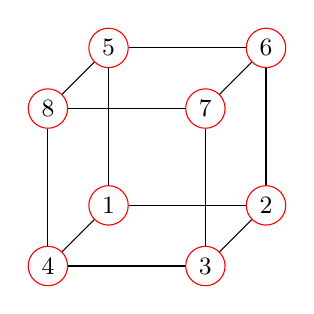
\begin{tikzpicture}
        % Define cube vertices
        \foreach \x/\y/\z/\n in {0/0/0/1, 2/0/0/2, 2/2/0/6, 0/2/0/5,
                                  0/0/2/4, 2/0/2/3, 2/2/2/7, 0/2/2/8} {
            \node[circle, draw=red, fill=white, minimum size=0.5cm, inner sep=0pt, font=\small] (\n) at (\x,\y,\z) {\n};
        }
        % Draw cube edges
        \foreach \a/\b in {1/2, 2/3, 3/4, 4/1,  % Bottom face
                           5/6, 6/7, 7/8, 8/5,  % Top face
                           1/5, 2/6, 3/7, 4/8}  % Connecting edges
        {   \draw (\a) -- (\b);}
    \end{tikzpicture}
    \end{center}
    Then for $n \geq 3$ we can get $P_n$ by going through the following cases: \\[2mm]
    \textbf{Case 1:} The ant is at the top for the $(n-2)$th and the $(n-1)$th moves, from which the ant will remain at the top with probability $1/2$ and the overall probability of this case is $ \frac{1}{2} \cdot P_{n-2} \cdot P_{n-1}$ \\[2mm]
    \textbf{Case 2:} The ant is at the top for the $(n-1)$th move, but at the bottom for the $(n-2)$th move, then at this point the $n$th move is guaranteed to be at the top too, the overall probability of this case is $P_{n-1}(1 - P_{n-2})$ \\[2mm] 
    \textbf{Case 3:} You are at the bottom for the $(n-2)$th and the $(n-1)$ moves, then similarly to the case 1, the overall probability of this case is $ \frac{1}{2} (1 - P_{n-2})(1 - P_{n-1})$ \\[3mm]
    \textbf{Case 4:} The ant is at the top for the $(n-2)$th move, but at the bottom for the $(n-1)$th move... then is simply impossible to get back to the top again, so the overall probability of this 'case' is 0. \\[2mm]
    Therefore
    \begin{align*}
        P_{n} &= \frac{ P_{n-2} \cdot P_{n-1} + (1 - P_{n-2})(1 - P_{n-1}) }{2} + P_{n-1}(1 - P_{n-2}) \\
        \iff P_n &= \frac{1 + P_{n-1} - P_{n-2}}{2}
    \end{align*}
    The best we can do is leave the answer as a recurrence, instead of getting the painful closed form of 
    \[
        P_n =
        \frac{
        (-11 \sqrt{7} + 7i) \left(\frac{1}{4} - \frac{i \sqrt{7}}{4}\right)^n
        - 2 (5 \sqrt{7} - 7i) \left(\frac{1}{4} + \frac{i \sqrt{7}}{4}\right)^n
        }{
        42 (\sqrt{7} - i)
        }
        + \frac{1}{2}
    \]
    $\Box$
\end{solution}

\begin{problem}[C][6][OTIS Mock AIME]
    % Counting ^ Expected Value
    Perry the Panda is eating some bamboo over a five-day period from Monday to Friday (inclusive). On Monday, he eats 14 pieces of bamboo. Each following day, Perry eats either one less than three times the previous day or one more than the previous day, with equal probability. Compute the expected number of pieces of bamboo Perry has eaten throughout the week after the end of Friday.
\end{problem}

\begin{solution}[434]
    Let $X$ be the number of pieces of bamboo eaten throughout the week, and let $X_1, X_2 \ldots, X_5$ be the number of pieces eaten each day, where $X_1$ corresponds to Monday, $X_2$ to Tuesday, and so on. It is obvious that $X = X_1 + X_2 + \ldots + X_5$. Then by linearity of expectation we have
    \begin{align*}
        \mathbb{E}(X_i) &= \frac{1}{2} \cdot \mathbb{E} (3X_{i-1} - 1) + \frac{1}{2} \cdot \mathbb{E}( X_{i-1}+1) \\
        &= \frac{3\mathbb{E}(X_{i-1}) - 1 + \mathbb{E}(X_{i-1}) + 1}{2} = 2 \mathbb{E} (X_{i-1})
    \end{align*}
    So the expected number of pieces eaten duplicates each day, starting from $X_1 = 14$, it must be the case that $\mathbb{E}(X_i) = 14 \cdot 2^{i-1}$. It follows that 
    \begin{align*}
        \mathbb{E}(X) = 14 (1 + 2 + 4 + 8 + 16) = 14(32-1) = 434
    \end{align*}
    $\Box$
\end{solution}

\begin{problem}[C][7][Mock AMC]
    % Counting ^ Stirling Numbers
    Mikaya has a list of $101$ Starbucks orders and would like to rank them relative to one another. Let $W$ be the number of ways she can order from worst to best, with ties allowed (multiple orders can be considered the same greatness). What is the remainder when $W$ is divided by $101$?
\end{problem}

\begin{solution}[1]
    Let $r_n$ be the number of ways to rank $n$ orders. Let $k$ be the number of orders in the first place, we can select them in $\binom{101}{k}$ different ways, then the rest can be arranged in $r_{101-k}$ ways. Summing over all $k$ we get 
    $$ r_{101} = \binom{101}{1}r_{100} + \binom{101}{2}r_{98} + \ldots + \binom{101}{101}r_0 $$
    But for any prime $p$, it is known that $p \mid \binom{p}{k}$ for $0 < k <p$, basically because the denominator is the multiplication of several factors less than $p$, it 'survives'. Our answer must be $r_{101} \hspace{-4pt} \mod{101} = r_0 = 1$ $\Box$
\end{solution}

\begin{solution}[(overkill)]
    We can make a ranking with $k$ levels in $k! \cdot \stirling{101}{k}$ ways. Where $\stirling{n}{k}$ corresponds to the Stirling numbers of the second kind, i.e, the number of ways to partition a set of size $n$ into $k$ non-ordered groups. We need then to compute $1!\stirling{101}{1} + 2!\stirling{101}{2} + \ldots + 101!\stirling{101}{101} \pmod{101}$. We will use the two following facts, we invite the reader to investigate why they work. \\[3mm]
    \textbf{Fact 1:} 
    $$ k! \cdot  \stirling{n}{k} = \sum_{i=1}^n(-1)^{k-i} \binom{k}{i} i^n$$
    \textbf{Fact 2:} For $k>1$ we have
    $$ k(x-1)^{k-1} = \sum_{i=0}^k (-1)^{k-i} \binom{k}{i} i x^{i-1}$$
    This can be obtained by implicit differentiation with the Binomial Theorem at $x=1$. \\[2mm]
    \textbf{Claim: } for $k > 1$, 101 divides $ k! \cdot \stirling{101}{k}$. \\
    This actually holds for any prime $p$, but we will focus at $p=101$. By Fermat's Little Theorem we have
    \begin{align*}
        k! \cdot  \stirling{101}{k} = \sum_{i=0}^{101}(-1)^{k-i} \binom{k}{i} i^{101} &\equiv   \sum_{i=0}^{101} (-1)^{k-i} \binom{k}{i} i \pmod{101} \\
        &\equiv  k \cdot (1-1)^{k-1} \equiv 0 \pmod{101}
    \end{align*}
    So we actually have all the terms being divisible by 101, except when $k=1$, then our answer must be $1! \cdot \stirling{101}{1} = \boxed{1}$
\end{solution}

\begin{problem}[C][8][Folklore]
    % Induction ^ Linear Algebra
    In a town, there are $n$ people and $k$ clubs. Each club has an odd number of members,
and any two clubs have an even number of common members. Prove that $k \le n$.
\end{problem}

\begin{solution}[(using induction)]
    We will prove that if we have $k$ clubs $C_1, C_2, \ldots, C_k$, such that, $|C_i|$ is odd and $|C_i \cap C_j|$ is even, then we have at least $k$ different people, also that every member has joined an odd amount of groups. By using induction, take the base case at $k=1$, then it is evident that we need to have at least one person, and that each person has joined an odd amount of groups; so we can assume that for any $r \leq k$ the argument is true. \\
    We will show that if it is true for $r \leq k$ then it is also true for $r+1$, let $C_{r+1}$ be the new club, we wish to show that this action implies the existence of at least two new persons (to maintain parity, it can't be only one). Assume by contradiction that all the club members of $C_{r+1}$ belong to another club, in other words, for each person $c \in C_{r+1}$, we also have $c \in C_v$ for some $v$. Now define $p(c)$ for each $c \in C_{r+1}$ as the amount of clubs different from $C_{r+1}$ to which $c$ belongs, from our hypothesis, $p(c)$ is odd. Now consider then the sum
    $$S = \sum_{c \in C_{r+1}} p(c) =|C_1 \cap C_{r+1}| + |C_2 \cap C_{r+1}| + \ldots + |C_r \cap C_{r+1}|$$
    Since each term of the form $|C_i \cap C_{r+1}|$ is even, $S$ must be even, but $S$ also is the sum of over all $p(c)$, since these elements are odd, and the size of $|C_{r+1}|$ is odd, $S$ must be odd, so this can't be possible unless our assumption was incorrect and there are elements that are only in $C_{r+1}$, these new elements are in an odd number of groups (only $C_{r+1}$), so the argument follows $\Box$
\end{solution}

\begin{problem}[C][9][Folklore]
   % Counting ^ Generating Functions ^ Discrete ^ Derivatives
\begin{enumerate} 
\item[\textbf{a)}] Let $S = \{1, 2, 3, 4, \dots, n\}$. Show the number of subsets $a \in S$ with an even sum of elements is equal to the number of subsets $b \in S$
with an odd sum of elements. 
\item[\textbf{b)}] Let $a \in S$ and $b \in S$ be defined as in the last problem. Let $\#(s)$ denote the sum of the elements of an arbitrary set $s$. Show \[\sum_{a \in S} \#(a) = \sum_{b \in S} \#(b).\]
\end{enumerate}
\end{problem}

%\begin{solution}
%\begin{enumerate}
%\item[\textbf{a)}] We'll write \( S \) as \( S_n \) to distinguish between subsets of different sizes and use \( \sum P \) to denote the sum of elements in set \(P\). The proof will be done with induction. 

%First, observe that the claim is true for \(n=1\). The subsets of \(S_1=\{1\}\) are \( \mathcal{P}(S_1) = \{\emptyset, \{1\}\}\). Since \( \sum\emptyset = 0 \) (even) and \( \sum\{1\} = 1 \) (odd), there is an equal number of subsets with even and odd sums.

%Now, assume the claim is true for \( n=k \). Thus, we have that set \( S_k \) has an equal number of subsets with even and odd sums. 

%Next, consider \( S_{k+1} = S_k\cup \{k+1\}\). For each subset \(P_i \subseteq S_k\), we'll now have subsets \( P_i,P'_i \subseteq S_{k+1} \), where \(P'_i = P_i \cup \{k+1\} \). Since subsets \(P_0, P_1, \dots\) are all the subsets of \( S_k \), they are already evenly split between even and odd sums. For subsets \(P_0', P_1', \dots\), they may change depending on if \(k+1\) is even or odd. If \(k+1\) is even, the even sums will remain even, and the odd sums will remain odd. If \( k+1 \) is odd, the even sums will become odd, and the odd sums will become even. In either case, there are still an equal number of odd and even sums. 

%Thus, by induction, the number of subsets $a \in S$ with an even sum of elements is equal to the number of subsets $b \in S$ with an odd sum of elements. 
%\end{enumerate}
%\end{solution}

\begin{solution} [(using bijection)]
    For any set $A$, define $A' = A \Delta \{1\}$ (the symmetric difference), that is :
    \begin{align*}
        A' = 
        \begin{cases}
            A \, \backslash \, \{ 1 \} & \text{If } 1 \in A \\
            A \, \cup \, \{ 1 \} & \text{If } 1 \notin A \\
        \end{cases}
    \end{align*}
    For part a), note that $\# A' = \#A \pm 1$, so if $\# A'$ is even, it implies that $\#A$ is odd, and vice versa. Now since $(A')' = A$, there's a one-to-one correspondence between the number of sets with even and odd sum. \\[3mm]
    As for part b), we need to show that the sum of $\#(a_0)$ over all subsets $a_0 \subseteq a$ is the same as the sum of $\#(b_0)$ over all subsets $b_0 \subseteq b$.
    
    Recall from part a) that there's a bijection between $s$ and $s'$ for any subset $s \subseteq S$, even better is the fact that if $s \subseteq a$, then $s' \subseteq b$ and since $\#s' - \#s$ is either 1 or \(-1\), we need to ensure that for each case that contributes a 1, there's a case that contributes a \(-1\). Indeed, $1 \in s \iff \#s' - \#s = -1$ and $1 \notin s \iff \#s' - \#s = 1$. Since the number of subsets that include 1 are equal to the numbers of subsets that do not include 1, we have a one-to-one correspondence and the claim follows $\Box$  \\[2mm]
    Note: Part a) can be concluded immediately by only using the argument of our last sentence. 
\end{solution}

\begin{solution}[(using generating functions)]
    Let $\mathcal{E} = \{ A \, | \, \#(A) \text{ is even } \}$ and $\mathcal{O} = \{ A \, | \, \#(A) \text{ is odd } \}$. Let's define a function $G$ as
    $$ G(x) = \prod_{i=0}^n (1 + x^i) = \sum_{s \subseteq S} x^{\#(s)}$$
    The most important fact about $G$ is that when expanded, the coefficient of $x^k$ counts the number of subsets whose elements sum to $k$. Also check that $G(-1) = G'(-1) =  0$. \\
    For part a) we need to show that $|\mathcal{E}| = |\mathcal{O}|$, then setting $x=-1$, we have 
    \begin{align*}
        0 = G(-1) = \sum_{s \subseteq S} (-1)^{\#(s)} = \sum_{s \subseteq \mathcal{E}} 1 + \sum_{s \subseteq \mathcal{O}} (-1) = |\mathcal{E}| - |\mathcal{O}| \\
        \iff |\mathcal{E}| = |\mathcal{O}| 
    \end{align*}
    As for part b), we use the first derivative of $G$: 
    $$ G'(x) = \sum_{s \subseteq S} \#(s) \cdot x^{\#(s) - 1}$$
    Then evaluating again at $x=-1$, gives us the desired result, similar to part a), since $G'(-1) = 0$ $\Box$
\end{solution}

\end{document}